\section{Versuchsaufbau}

Die hier verwendeten GaAs Proben sind nur im Infraroten halbwegs durchlässig, weshalb ein
Infrarot-Messplatz eingerichtet wird, welcher in Abbildung \ref{fig:aufbau} dargestellt ist.

\begin{figure}[H]
  \centering
  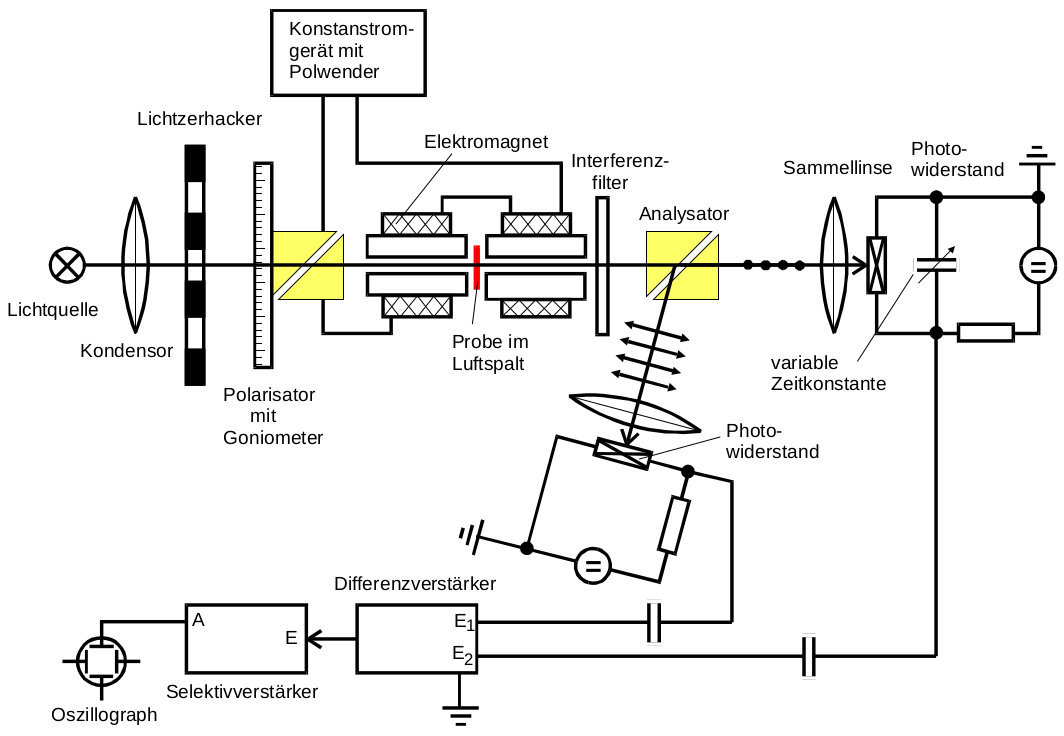
\includegraphics[width=11cm]{Aufbau.png}
  \caption{Aufbau der verwendetem Messapparatur.}
  \label{fig:aufbau}
\end{figure}

Als Lichtquelle wird eine Halogen-Lampe verwendet, da ihr Emissionsspektrum im Infraroten liegt.
Das emittierte Licht wird zunächst mithilfe einer Sammellinse fokussiert und anschließend durch
den "Lichtzerhacker" geleitet. Das noch unpolarisierte Licht wird nun durch ein Glan-Thomson-Prisma
linear polarisiert und fällt anschließend auf die Probe, welche sich im Magnetfeld eines
Elektromagneten befindet.
Bevor die austretende Strahlung detektiert wird, wird sie mithilfe eines Interferenzfilters monochromatisiert,
um den Faraday-Effekt wellenlängenabhängig zu untersuchen. Durch ein weiteres Glan-Thomson-Prisma wird der
Strahl in zwei Strahlen geteilt, welche senkrecht zueinander polarisiert sind. Die Intensität der beiden
Strahlen wird unabhängig voneinander durch zwei Photowiderstände aus PbS gemessen. Ihr Innenwiderstand ist
proportional zur Lichtintensität, jedoch kommt es aufgrund der hohen Innenwiderstandes zu Rausspannungen.
Um diese zu minimieren wird die Wechsellichtmethode verwendet, welche durch den "Lichtzerhacker" am Anfang des
Strahlengangs ermöglicht wird. Diese rotierende Sektorscheibe zerhackt das Licht in gleichmäßige Impulse, wodurch
an den Photodioden ein Wechselstrom messbar wird. Die Spannungen werden auf einen Differenzverstärker und anschließend auf
einen Selektivverstärker gegeben um das Signal auf einem Oszilloskop sichtbar zu machen.
Die Differenz der beiden Signale verschwindet genau dann, wenn beide Eingangssignale nach Betrag und Phase
übereinstimmen.


\section{Durchführung}
Zunächst wird das Magnetfeld mithilfe einer Hall-Sonde, welche auf der optischen Achse montiert werden kann, vermessen.
Um das Maximum zu bestimmen, wird die Hallsonde langsam durch den Elektromagneten bewegt.
Um die Faraday-Rotation zu vermessen, muss die Apparatur zunächst justiert werden. Dabei muss beachtet werden, dass
die beiden geteilten Strahlen exakt auf die Detektorflächen der Photodioden treffen.
Ist dies geschehen, wird die Faraday-Rotation für zwei n-dotierte GaAs Proben und eine reine GaAs Probe vermessen dessen
Eigenschaften in der folgenden Tabelle aufgeführt sind.

\begin{table}[H]
  \centering
  \caption{Eigenschaften der Proben.}
  \label{tab:tabe6}
    \begin{tabular}{l l l}
    \toprule
    Probe & Dotierung N $\SI{e18}{\per\cubic\cm}$ & L/mm\\
    \midrule
    1 & 1,2 & 1,36\\
    2 & 2,8 & 1,296\\
    3& - & 5,11\\


          \bottomrule
        \end{tabular}
    \end{table}


Die Faraday-Rotation wird mithilfe des Polarisators vor dem Elektromagneten bestimmt. Dazu wird der Winkel am Polarisator notiert,
für den die Signalamplitude auf nahezu Null abfällt. Anschließend wird das Magnetfeld umgepolt und der Winkel erneut vermessen.
Dieses Vorgehen wird für jede Probe mit 9 Interferenzfiltern von 1,06\;$\symup{\mu}$m bis 2,65\;$\symup{\mu}$m  wiederholt.
